\chapter{Introduction to Practical Antenna}
\verb|	So| far, we have discussed the Hertz dipole, then the finite length dipole, an extension of the Hertz dipole, which we called the thin wire dipole. Also, we discussed general characteristics of antennas like directivity, effective aperture, half-power beam width, radiation pattern and so on. Now we will be discussing some practical antennas which are used at low-frequency UHF and VHF band\footnote{Very High Frequency(VHF), Ultra High Frequency(UHF)} that lie in the category of dipole antennas. It is important to note that at low frequencies the dipole size becomes excessively large since the length of the dipole should be to some extent comparable to the wavelength for substantial radiation which is an important factor for the choice of antennas.


\section{Monopole Antenna}The monopole antenna is used for medium wave broadcasting and they are present in radio stations. The monopole is essentially half of a dipole erected over an ideal ground surface.

We have seen that at lower frequencies, a medium with low conductivity starts behaving like a good conductor. Precisely, this is what happens for the earth medium, at lower frequencies, it becomes more like a conductor and then an antenna can be erected over it and it behaves as if the antenna was mounted on an ideal conducting surface. The dipole antenna is inapplicable at medium-frequency signals because as it was stated earlier, the antenna size becomes large at this frequency.

We will analyze the monopole antenna using the concept of image. Let's consider a charge over a conducting surface as shown in Figure 50.1 and we will examine the field produced by this charge as it interacts with the conducting surface(ideal ground surface). We will observe that at the conducting surface the fields are perpendicular to it as it goes to zero (no charges on the conducting surface). This is equivalent to a negative charge below the conducting surface at the same distance as the charge above it when the conducting surface is removed. 
%Diagram
\begin{figure}[h]
\centering
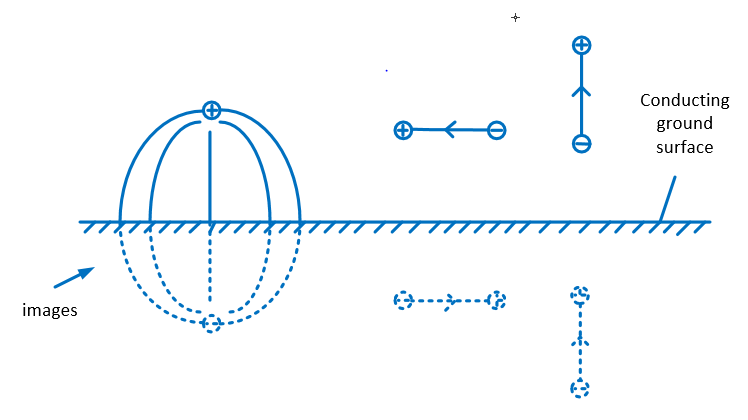
\includegraphics[height=5cm]{./graphics/image53_1}
\caption{Concept of Images}
\label{fig:fig50.1}
\end{figure}

Also, if we have a current flowing towards the left which is equivalent to accumulation of positive charges to the left and negative charges to the right, then the image would be flowing towards the right as shown and also for a current flowing upward the image is shown to also flow in the same direction because the image of the negative charge closest to the conducting surface is a positive charge and the image of the positive charge farthest to the conducting plane is a negative charge which still produces current in the same direction as the original current. So what we observe is that if we have a charge, then the image has opposite polarity and for a current flowing parallel to the conducting surface, the image flows in the opposite direction. However for a current flowing vertically to the conducting surface the image has no 180\textdegree \space shift essentially the image flows in the same direction. The concept of images applied to a charge or current located over the ground plane is replacing the ground plane by the corresponding images. We have seen the current distribution on the dipole antenna as shown in Figure 50.2a and it is symmetric about the centre (feed point) and both lines from the centre are equal in length. This structure is similar to a ground plane with monopole and its behaviour (radiation characteristics) is identical to that of the dipole antenna except for some differences which we will observe.

\begin{figure}[h]
\centering
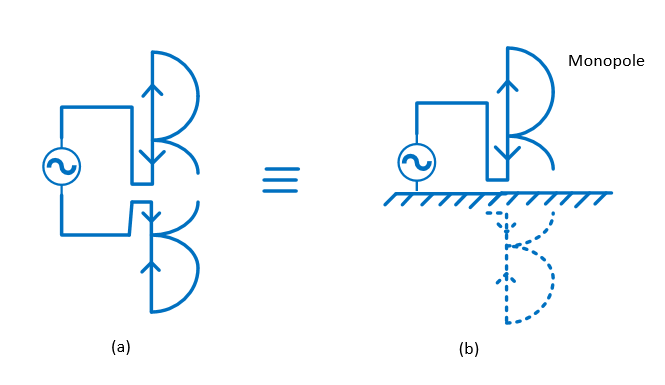
\includegraphics[height=5cm]{./graphics/image53_2}
\caption{a. the current distribution of a dipole 
	b. the current distribution of a monopole with it image below the conducting surface.}
\label{fig:fig2}
\end{figure}

Now let's note some facts between the two antennas shown in Figure 50.2a and 50.2b
\begin{enumerate}[(i)]
\item The radiation pattern of the monopole is similar to that of the dipole because the monopole antenna is similar to having another current element, located below the surface however, there is no radiation pattern below the surface as it is a conductor so energy does not propagate inside the conductor. So the monopole has radiation in a semi-infinite space which is the upper half of the radiation pattern of a dipole.
\item The monopole has half the power radiated compared to the dipole since the radiation is in semi-infinite space for the same current in the dipole with infinite space.
\item Also, since power radiated is proportional to the radiation resistance for a given current, the monopole has a terminal impedance or radiation resistance which is half that of the dipole antenna.
\end{enumerate}
So with these facts, we can conclude that the fields for the monopole is identical to that of the dipole and also the radiation pattern would be symmetrical about the $\phi$ direction which is the case of the dipole. Precisely this is one of the reasons the monopole antenna is used for low frequency radio broadcasting because the radiation pattern is symmetric on the ground as shown in Figure 50.4. So if we consider a dipole length of less than $\lambda$ for instance, we know there is only one maximum which is shown in Figure 50.4 and it is on the ground oriented in the $\phi$ direction. Also, as we go to higher heights the amplitude of the electric field dies down. This means the antenna is most suited to have radiation on the ground surface which is the purpose in broadcasting.

The next important reason which have been stated before is that at medium frequency the wavelength is typically in the order of a few hundred meters so the size of the dipole antenna is very large and if it were to be mounted to avoid the ground effect it would be mounted at a significant height. On the contrary, the monopole antenna is mounted on the ground vertically and the radiation pattern is symmetrical on the ground.
%Diagram
\begin{figure}[h]
\centering
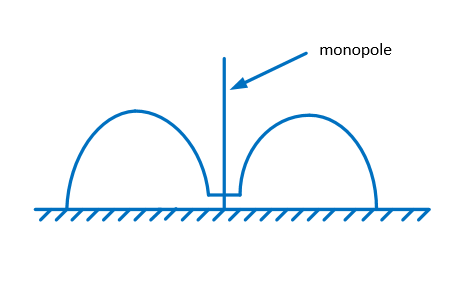
\includegraphics[height=5cm]{./graphics/image53_3}
\caption{Radiation pattern of a monopole of length, less than a wavelength i.e $l < \lambda$}
\label{fig:fig3}
\end{figure}

However, as we go to higher frequencies, the antenna size becomes small and it becomes possible to effectively use the dipole antennas, because the wavelength is now in the range of a few meters, like TV signals. Also, the length of the dipole is typically taken as $\dfrac{\lambda}{2}$; which is the most commonly used dipole because its radiation resistance is 73$\Omega$, which is very near the 50$\Omega$ or 75$\Omega$ characteristic impedance of some transmission lines. This is one of the properties we will examine while analyzing this dipole in the next section.
\section{$\dfrac{\lambda}{2}$ Dipole}
The $\dfrac{\lambda}{2}$ Dipole with it current distribution is shown in Figure 50.4 which has maximum current at the center.
%Diagram
\begin{figure}[h]
\centering
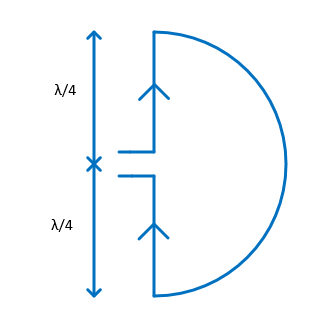
\includegraphics[height=5cm]{./graphics/image53_4}
\caption{Dipole Antenna}
\label{fig:fig4}
\end{figure}
Lets write the expression for the electric field from equation \ref{eqn12} given as; 
\begin{equation*}
E_\theta = j60I_m \frac{F(\theta)e^{jBr}}{r}
\end{equation*}
\begin{center}
Also, the radiation pattern $F(\theta)$ is given as $\dfrac{cos(\beta H cos\theta) - cos\theta H}{sin \theta}$

For the case of the $\dfrac{\lambda}{2}$ dipole, $H = \dfrac{\lambda}{4}$ so $\beta H = \dfrac{2\pi}{\lambda} \times \dfrac{\lambda}{4}= \dfrac{\pi}{4} $ which reduces $F(\theta)$ to;

$F(\theta) = \dfrac{cos (\dfrac{\pi}{2} cos\theta)}{sin\theta}$

Then, $E_\theta = j60I_m \dfrac{cos (\dfrac{\pi}{2} cos\theta)}{sin\theta} \dfrac{e^{jBr}}{r}$ 
\end{center}for the half wavelength dipole.
Taking the limits of $F(\theta)$ at $\theta = 0$ or $\pi$ shows that the radiation pattern has nulls at $\theta = 0 \text{ or } \pi$ and also has a maximum at $\theta = \dfrac{\pi}{2} (sin \dfrac{\pi}{2} = 1)$ which is similar to the radiation pattern of the Hertzian Dipole.

Next, lets find the total power radiated by this half-wavelength dipole and the radiation resistance. 
\[ \text{We know; Power radiation } W = \int_0^{2\pi}\int_{0}^{\pi} \frac{1}{2}\frac{|E_\theta|^2}{n}r^2sin\theta d\theta d\phi \]
\[ = (2\pi)\int_{0}^{\pi} \frac{1}{2} 60^2 \frac{I_m^2cos^2(\frac{\pi}{2}cos\theta)}{\eta sin^2\theta}sin\theta d\theta \]

\[ W = \frac{60^2\pi}{\eta} I_m^2 \int_{0}^{\pi} \frac{cos^2(\frac{\pi}{2}cos\theta)}{sin\theta}d\theta \]
\[Recall\ \eta = 120\pi \]
\[ = 30I_m^2 \int_{0}^{\pi}\dfrac{cos^2(\frac{\pi}{2}cos\theta)}{sin\theta}d\theta \]
The integral can not be solved analytically so instead it is solved numerically to give a value of 1.218.
\[ \text{So } W = 30I_m^2 \times 1.218 \]
\begin{equation}
W = 36.54I_m^2
\end{equation}
$I_m$ is the maximum current which is shown by the current distribution at the center of the $\dfrac{\lambda}{2}$ dipole.
Also, the power that is radiated by the antenna is given as $$\dfrac{1}{2}I_m^2 R_{rad} = 36.54I_m^2$$
\[ \Rightarrow R_{rad} \approx 73.1\Omega \]
Generally, the dipole would have reactive fields which gives some resistance. In order to maintain a $73\Omega$ impedance at the input of the antenna, the reactive part is tuned by shortening the antenna length by a small amount. So in practice, the half-wavelength dipole is not exactly $\dfrac{\lambda}{2}$ but is $0.47\lambda$ which is a little shorter than $0.5\lambda$ and the reactive part is cancelled out. So the length of $0.47\lambda$ gives an input impedance $Z_{in}$ which is at most real and it is equal to the radiation resistance which is 73Ohms. Essentially, the choice of a $\dfrac{\lambda}{2}$ dipole is so that we get a $73\Omega$ impedance which nearly matches the $50\Omega$ or $75\Omega$ cables.

Next, we will calculate the half power beam width which is the width at the 3dB point on the radiation pattern as shown in Figure 50.6.
\[ F(\theta) = \dfrac{cos(\dfrac{\pi}{2}cos\theta)}{sin\theta} = \dfrac{1}{\sqrt{2}} \]
\[ = \sqrt{2}cos(\dfrac{\pi}{2}cos\theta) = sin\theta \]
\[ \theta_{HP} \approx 78\text{\textdegree} \]
%diagram
\begin{figure}[h]
\centering
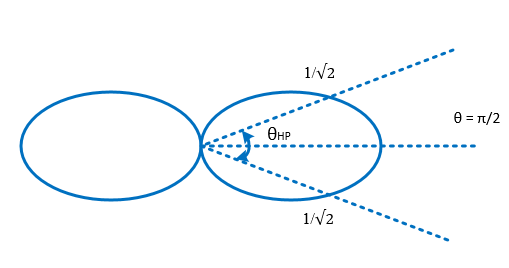
\includegraphics[height=5cm]{./graphics/image53_5}
\caption{Radiation pattern of a Hertz Dipole}
\label{fig:fig5}
\end{figure}

For the Hertz dipole, given that the radiation pattern is $sin\theta$, then the half power points is 90\textdegree($\theta_{HP} = 90\text{\textdegree}$). As we translate from the Hertz dipole to the half-wavelength dipole, the angle reduces from 90\textdegree to 78\textdegree  which means the antenna becomes narrower. Also, the same scenario occurs if the length is changed from $\dfrac{\lambda}{2}$ to $\lambda$ which is, the radiation pattern remains the same but the beam width becomes smaller and the antenna become more directive.

Lets find the directivity of the half-wavelength dipole given 
\[ \text{Directivity }D = \dfrac{4\pi}{\int_{0}^{2\pi}\int_{0}^{\pi}|E_n(\theta ,\phi)|^2sin\theta d\theta d\phi} \]
\[ = \dfrac{4\pi}{\int_{0}^{2\pi}\int_{0}^{\pi}\dfrac{cos^2(\frac{\pi}{2}cos\theta)}{sin^2\theta}sin\theta d\theta d\phi} = \dfrac{4\pi}{\int_{0}^{2\pi}\int_{0}^{\pi}\dfrac{cos^2(\frac{\pi}{2}cos\theta)}{sin\theta} d\theta d\phi} \]
\[ = \dfrac{4\pi}{2\pi\int_{0}^{\pi}\dfrac{cos^2(\frac{\pi}{2}cos\theta)}{sin^2\theta}sin\theta d\theta d\phi} = \dfrac{2}{1.218} \approx 1.64 \]
\[ \text{Directivity in dB } = 10log1.64 \approx 2.15dB \]
This means that for the half-wavelength dipole, the power density in the perpendicular direction to the dipole is 2.15dB higher compared to an isotropic antenna.

Next, we calculate the effective aperture which is given as 
\[A_e = \dfrac{\lambda^2 D}{4\pi} = \dfrac{1.64\lambda^2}{4\pi} \approx 0.13\lambda^2 \]

\section{$\dfrac{\lambda}{4}$ Monopole Antenna}
\begin{figure}[h]
\centering
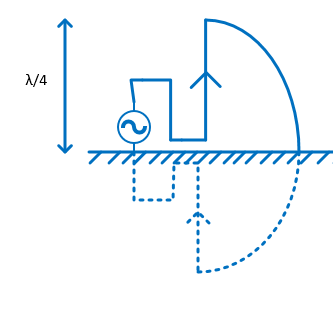
\includegraphics[height=5cm]{./graphics/image53_7}
\caption{Monopole Antenna}
\label{fig:fig7}
\end{figure}
\begin{equation*}
\text{Recall that }E_\theta = j60I_m \frac{F(\theta)e^{jBr}}{r}
\end{equation*}
\begin{center}
Also, the radiation pattern $F(\theta)$ is given as $\dfrac{cos(\beta H cos\theta) - cos\theta H}{sin \theta}$

For the case of the $\dfrac{\lambda}{4}$ monopole, $H = \dfrac{\lambda}{4}$ so $\beta = \dfrac{2\pi}{\lambda} \times \dfrac{\lambda}{4}$

$ = \dfrac{\pi}{4} $ which reduces $F(\theta)$ to; $F(\theta) = \dfrac{cos (\dfrac{\pi}{2} cos\theta)}{sin\theta}$

Then, $E_\theta = j60I_m \dfrac{cos (\dfrac{\pi}{2} cos\theta)}{sin\theta} \dfrac{e^{jBr}}{r}$ for the quarter wavelength monopole.
\end{center}
Next, let's find the total power radiated by this quarter-wavelength monopole and the radiation resistance. 
\[ \text{We know; Power radiation } W = \int_0^{2\pi}\int_{0}^{\frac{\pi}{2}} \frac{1}{2}\frac{|E_\theta|^2}{\eta}r^2sin\theta d\theta d\phi \]
\[ = (2\pi)\int_{0}^{\frac{\pi}{2}} \frac{1}{2} 60^2 \frac{I_m^2cos^2(\frac{\pi}{2}cos\theta)}{\eta sin^2\theta}sin\theta d\theta \]
$$\text{since}\ |e^{-j\beta r}| = \sqrt{\cos^2(\beta r) + \sin^2(\beta r)} = 1.$$
\[ W = \frac{60^2\pi}{\eta} I_m^2 \int_{0}^{\frac{\pi}{2}} \frac{cos^2(\frac{\pi}{2}cos\theta)}{sin\theta}d\theta \]
\[ \eta = 120\pi \]
\[ = 30I_m^2 \int_{0}^{\frac{\pi}{2}}\dfrac{cos^2(\frac{\pi}{2}cos\theta)}{sin\theta}d\theta \]

The integral can not be solved analytically so instead it is solved numerically to give a value of 0.69.
\[ \text{So } W = 30I_m^2 \times 0.69 \]
\begin{equation}
W = 18.28I_m^2
\end{equation}
Also, the power that is radiated by the antenna is given as $\dfrac{1}{2}I_m^2 R_{rad} = 18.28I_m^2$
\[ \Rightarrow R_{rad} \approx 36.55\Omega \]

Let's find the directivity of the quarter-wavelength monopole given 
\[ \text{Directivity }D = \dfrac{4\pi}{\int_{0}^{2\pi}\int_{0}^{\frac{\pi}{2}}|E_n(\theta\phi)|^2sin\theta d\theta d\phi} \]
\[ = \dfrac{4\pi}{\int_{0}^{2\pi}\int_{0}^{\frac{\pi}{2}}\dfrac{cos^2(\frac{\pi}{2}cos\theta)}{sin^2\theta}sin\theta d\theta d\phi} = \dfrac{4\pi}{\int_{0}^{2\pi}\int_{0}^{\frac{\pi}{2}}\dfrac{cos^2(\frac{\pi}{2}cos\theta)}{sin\theta} d\theta d\phi} \]
\[ = \dfrac{4\pi}{2\pi\int_{0}^{\frac{\pi}{2}}\dfrac{cos^2(\frac{\pi}{2}cos\theta)}{sin^2\theta}sin\theta d\theta d\phi} = \dfrac{2}{0.69} \approx 3.28 \]
\[ \text{Directivity in dB } = 10log3.28 \approx 5.15dB \]

Next, we calculate the effective aperture which is given as 
\[ \dfrac{\lambda^2 D}{4\pi} = \dfrac{3.28\lambda^2}{4\pi} \approx 0.26\lambda^2 \]

%\paragraph{Practice Question}
%Consider a quarter-wavelength monopole and derive the characteristics that was derived for the half wavelength dipole.